\chapter{Introduction}

In last decades Information Technology has been the main topic in most
research centers of the world. Human-Computer interaction is becoming
more and more an easy available technology in everyday life. This thanks
to impressive advancements in research topics like Machine learning, Automatic
Speech Recognition and Understanding, Data-driven stochastic
approaches, Text Processing and Speech Synthesis.
\par
One class of applications relying heavily on this technologies is Spoken
Dialog Systems. Spoken Dialog Systems allow humans to engage complex
dialogs with machines using the most natural communication mean ever
known: their voice. In the last decades, this class of applications has
been made able to interact with humans and satisfy their needs in such
a way that allows hoping that this technology will be soon available to
everybody and in any kind of device, from the most powerful desktop PC
to the cheapest laptops and mobile phones.

\section{Overview}
Spoken Language Understanding (SLU) is the semantic interpretation of
signs conveyed by a speech signal. The goal of SLU is to extract a conceptual
representation from spoken sentence transcriptions in a natural
language. This task is very complex. Signs to be used to produce conceptual
representation are coded in the signal along with other noisy information.
Spoken sentences many times don’t follow the grammar of a
language, they could contain self correction, hesitations, repetitions and
many other irregular phenomena due to the spontaneous nature of spoken
language. Furthermore SLU systems are applied to the output of an Automatic
Speech Recognizer (ASR) so they must be robust to noise introduced
by spontaneous events typical of spoken language and errors introduced by
ASR. ASR components produce a stream of words with no information
about sentence structure, like punctuation and sentence boundaries, so
SLU systems must perform text segmentation and understanding at the
same time. The level of complexity needed in order to represent the meaning
of a spoken utterance depends mainly on the application targeted.
\par
\begin{figure}
	\centering
	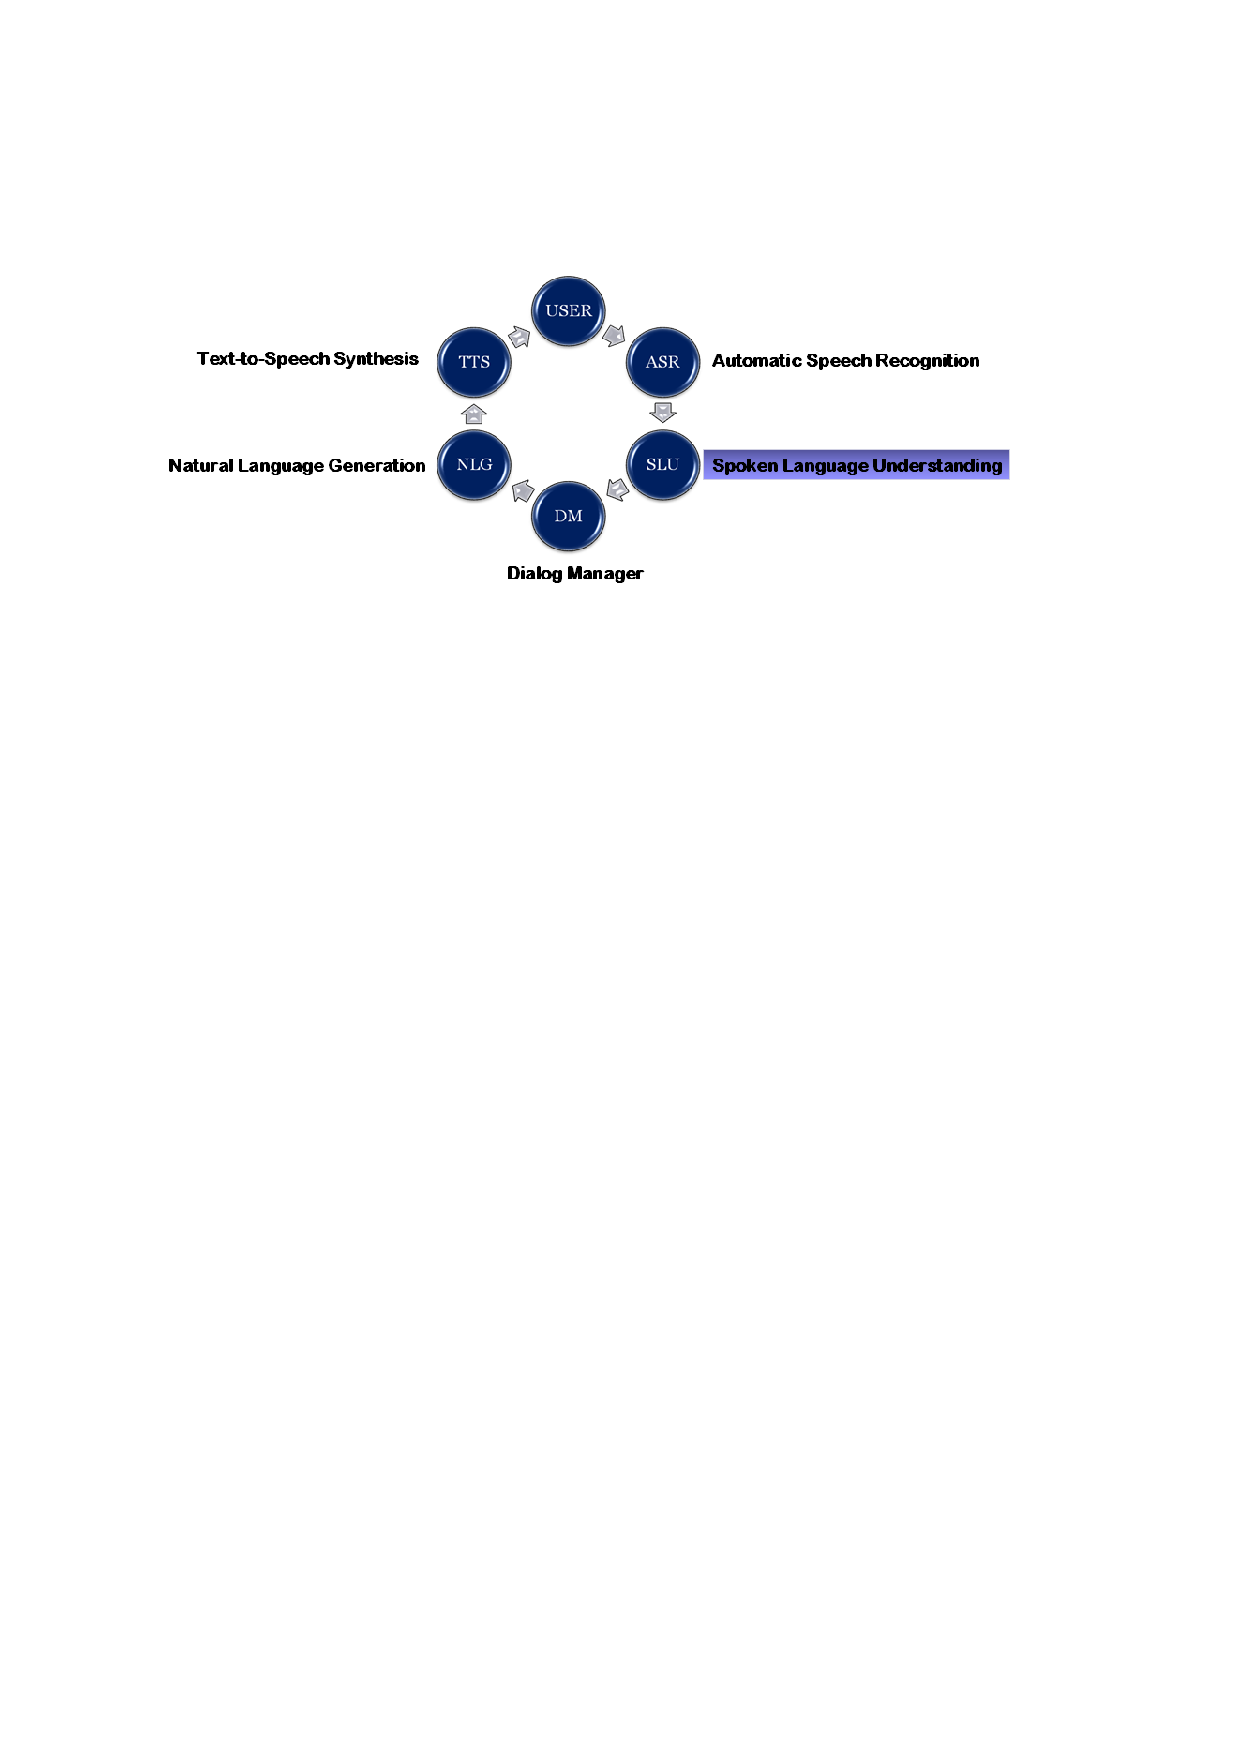
\includegraphics[width=\textwidth]{intro-cyclefig}
	\caption{High Level Depiction of Spoken Dialog Systems}
\end{figure}
The application we consider is Spoken Dialog, in particular we focus
on the understanding module of this class of applications. A high level
schema of a Spoken Dialog System application is shown in Figure 2.1. The
dialog is initiated by the user as response to an opening prompt from the
system. The user utterance is automatically transcribed by the Automatic
Speech Recognition (ASR) component. The ASR takes as input a speech
signal and produces its transcription in textual format. The Spoken Language
Understanding (SLU) module takes as input the output of ASR and
generates a meaning representation. Based on the interpretation coming
from the SLU module, the Dialog Manager (DM) select the next dialog
turn, this is converted into a natural language sentence by the Natural
Language Generation (NLG) module. Finally, the Text-To-Speech (TTS)
module synthsizes the generated sentence as a speech signal, which is sent
back to the user to continue the dialog. The loop depicted in Figure 2.1 is
repeated until the application completes the modelled task.
\par
Spoken dialog systems need sophisticated SLU models in order to implement
dialog applications that go beyond solving simple tasks like call
routing or form filling [35]. Three level of complexity can be defined for
dialog applications. The first level involves the translation from words to
basic conceptual constituents. The second level includes semantic composition on the basic constituents yielded in the first level. At the third level
context-sensitive validation is performed. At this level each utterance is
considered as a set of sub-utterances and a broad context is taken into
account. The interpretation of a sub-utterance is performed context sensitive
to the others. Going from level one to level three, tasks of increasing
complexity can be solved, from call routing or classification of utterances
[35] to Help-Desk application for hardware and software repairing [31].
\par
SLU is performed as a semantic parsing of spoken sentences. Approaches
based on syntactic analysis or directly on semantic analysis have been proposed,
in any case semantic constituents are instantiated by one or more
words that have a corresponding syntactic constituent. Among understanding
modules proposed in the last two decades, first solutions were
based on semantic grammars, but as the amount of data available for application
development increased, as well as application complexity, stochastic
approaches have been preferred.
\par
Many problems of interpretation in SLU systems derive from the fact
that many sentences are ungrammatical and ASR hypotheses contain errors,
so grammars have a limited coverage. These considerations suggest
the use of more specific, but more robust, models. In the early nineties,
the DARPA ATIS project started a series of task-dependent SLU systems.
Data were collected in the domain of a flight information and reservation
service. ATIS project aimed at providing a natural language interface to
a travel information database and provided a benchmark for many spoken
language understanding systems, one is discussed in [64].

\section{Objectives of this work}
Major components in SLU systems include identifying speaker’s intent and extracting semantic constituents from the natural language query, two tasks that are often referred
to as intent detection and slot filling. Intent detection can be treated as a semantic
utterance classification problem, and slot filling can be treated as a sequence labeling task.
These two tasks are usually processed separately by different models. For intent detection, a
number of standard classifiers can be applied, such as support vector machines (SVMs) and convolutional neural networks(CNNs). For slot filling, popular approaches include using sequence models such as maximum entropy Markov models (MEMMs), conditional random fields (CRFs), and recurrent neural networks (RNNs).
\par
Recently, neural network based models that jointly perform intent detection and slot filling
have been reported using CRF for joint intent detection and slot filling and recursive neural network (RecNN) that learns hierarchical representations of the input text for the
joint task. Such joint models simplify SLU systems, as only one model needs to be trained and
deployed.
\par
The previously proposed joint SLU models, however, are unsuitable for online tasks where it
is desired to produce outputs as the input sequence arrives. In speech recognition, instead of receiving the transcribed text at the end of the speech, users typically prefer to see the ongoing transcription while speaking. In spoken language understanding, with real time intent identification and semantic constituents extraction, the downstream systems
will be able to perform corresponding search
or query while the user dictates. The joint SLU
models proposed in previous work typically require
intent and slot label predictions to be conditioned
on the entire transcribed word sequence.
This limits the usage of these models in the online
setting.
\par
In this paper, we propose an RNN-based online joint SLU model that performs intent detection
and slot filling as the input word arrives. Therefore, we propose to perform intent detection,
slot filling, and language modeling jointly in a conditional RNN model. The proposed joint
model can be further extended for belief tracking in dialogue systems when considering the dialogue history beyond the current utterance. Moreover, it can be used as the RNN decoder in an end-to-end trainable sequence-to-sequence speech recognition model.